% Relatório - Sensor de distância por infravermelho (TCRT5000)
% Projeto de Sistemas Robóticos - DCC/UFMG - 2026/2
% Compilar com: pdflatex relatorio.tex (duas vezes, para as referências cruzadas)

\documentclass[11pt,a4paper]{article}

\usepackage[T1]{fontenc}
\usepackage[utf8]{inputenc}
\usepackage[provide=*,brazilian]{babel}
\usepackage{lmodern}
\usepackage{microtype}
\usepackage[a4paper,margin=2.5cm]{geometry}
\usepackage{amsmath}
\usepackage{icomma}
\usepackage{graphicx}
\usepackage{float}
\usepackage{booktabs}
\usepackage{tabularx}
\usepackage{array}
\usepackage[font=small,labelfont=bf]{caption}
\usepackage{enumitem}
\usepackage{xcolor}
\usepackage{listings}
\usepackage[american]{circuitikz}
\usepackage[hidelinks]{hyperref}

\graphicspath{{figuras/}}
\setlist{itemsep=2pt,topsep=4pt}
\setlength{\parskip}{4pt}

\newcommand{\cod}[1]{\texttt{#1}}
\newcommand{\cont}{\,\text{cont}^{1/2}}

\lstset{
  language=C++,
  basicstyle=\ttfamily\footnotesize,
  keywordstyle=\color{blue!60!black}\bfseries,
  commentstyle=\color{green!40!black}\itshape,
  stringstyle=\color{red!60!black},
  numbers=left, numberstyle=\tiny\color{gray}, numbersep=6pt,
  frame=single, rulecolor=\color{gray!50},
  breaklines=true, columns=fullflexible, keepspaces=true,
  literate={á}{{\'a}}1 {é}{{\'e}}1 {í}{{\'i}}1 {ó}{{\'o}}1 {ú}{{\'u}}1 {ã}{{\~a}}1 {õ}{{\~o}}1 {ç}{{\c{c}}}1 {â}{{\^a}}1 {ê}{{\^e}}1 {ô}{{\^o}}1
}

\begin{document}

% ------------------------------------------------------------------ capa
\begin{titlepage}
\centering
{\large Universidade Federal de Minas Gerais\par}
{\large Instituto de Ciências Exatas --- Departamento de Ciência da Computação\par}
\vspace{0.4cm}
{Projeto de Sistemas Robóticos --- 2026/2 --- Prof.\ Paulo Rezeck\par}
\vspace{3.5cm}
{\LARGE\bfseries Sensor de distância por infravermelho:\par}
\vspace{0.2cm}
{\Large caracterização e calibração do TCRT5000\par}
\vspace{0.6cm}
{\large Relatório da Aula 13\par}
\vspace{3cm}
{\large Equipe RTech Tabajara\par}
\vspace{0.6cm}
\begin{tabular}{ll}
\toprule
Integrante & Matrícula \\
\midrule
Guilherme Novais de Souza & 2022036047 \\
Hector Julio Pardinho Soares & 2017108353 \\
Lean Henrique Pereira Miranda & 2022035652 \\
Luís Eduardo Jorge Almeida & 2022423440 \\
Marcus Vinicius Gomes de Oliveira & 2022036152 \\
\bottomrule
\end{tabular}
\vfill
{Belo Horizonte, 2026\par}
\end{titlepage}

% ------------------------------------------------------------------ 1
\section{Introdução}

Calibramos o TCRT5000 como sensor de distância de 0 a 200~mm e embarcamos o modelo no Arduino. Os ganhos gravados no firmware foram $g_0 = 3{,}22$~mm e $g_1 = 306{,}2$~mm$\cdot$cont$^{1/2}$. Com eles, a estimativa erra 8,6~mm (RMSE) entre 20 e 180~mm. O sinal se separou do fundo até 200~mm, mas só por 1 a 2 contagens, e as leituras foram confiáveis até cerca de 160~mm.

O TCRT5000 reúne um LED infravermelho (cerca de 950~nm) e um fototransistor com filtro para luz visível. A luz emitida reflete no alvo, e parte dela volta ao detector. Quanto mais perto e mais claro o alvo, maior a corrente no coletor e menor a tensão lida no pino A0. A distância só aparece quando um modelo inverte essa curva.

Seguimos o roteiro da Aula 13 com quatro objetivos:
\begin{enumerate}
  \item medir o sinal em distâncias conhecidas, de 0 a 200~mm;
  \item ajustar o modelo inverso $d = g_0 + g_1/\sqrt{S}$;
  \item gravá-lo no Arduino, para que o sketch imprima o sinal e a distância em milímetros;
  \item avaliar o alcance e o efeito de reduzir os tempos de acionamento do LED.
\end{enumerate}

% ------------------------------------------------------------------ 2
\section{Materiais e montagem}

Montamos o circuito do roteiro com uma única troca de resistor (Tabela~\ref{tab:materiais}).

\begin{table}[!htb]
\centering
\caption{Materiais e função de cada item.}
\label{tab:materiais}
\begin{tabularx}{\textwidth}{>{\raggedright\arraybackslash}p{4.6cm}X}
\toprule
Item & Uso \\
\midrule
Arduino Mega 2560 & alimentação de 5~V, saída digital D8 e entrada analógica A0 (10 bits, 0 a 1023) \\
TCRT5000 & emissor e detector, montados na protoboard com a face voltada para cima \\
Resistor de 100~$\Omega$ & do D8 ao anodo do LED; limita a corrente do emissor a cerca de 38~mA com o D8 em nível alto \\
Dois resistores de 2~k$\Omega$ em série (4,0~k$\Omega$) & \emph{pull-up} do coletor ao 5~V, lido no A0, no lugar do resistor de 4,7~k$\Omega$ indicado \\
Régua transparente de 20~cm & fixada na vertical, com o zero na face do sensor \\
Alvo & placa branca impressa em PLA (base do braço mecânico das aulas anteriores), paralela à face do sensor \\
\bottomrule
\end{tabularx}
\end{table}

Com o \emph{pull-up}, o coletor fica perto de 5~V quando não chega luz infravermelha. A luz refletida faz o fototransistor conduzir, e a tensão em A0 cai. O D8 liga e desliga o emissor para separar a reflexão da luz ambiente. O sinal usado em todo o trabalho é
\begin{equation}
  S = \max\left(0,\ \mathrm{adc}_{\mathrm{off}} - \mathrm{adc}_{\mathrm{on}}\right).
  \label{eq:sinal}
\end{equation}

A Figura~\ref{fig:esquema} mostra o circuito. Com o D8 em nível alto, a corrente de cerca de 38~mA no resistor de 100~$\Omega$ corresponde a uma queda de aproximadamente 1,2~V no LED ($I = (5 - V_F)/100~\Omega$). O LED dissipa então cerca de 46~mW e o resistor, cerca de 0,14~W, durante o tempo em que fica aceso.

O \emph{pull-up} de 4,0~k$\Omega$ é cerca de 15\% menor que o de 4,7~k$\Omega$. Para a mesma corrente de coletor, a queda em A0 é proporcional ao resistor, então o sinal tende a sair menor na mesma proporção.

\begin{figure}[!htb]
  \centering
  \begin{circuitikz}[scale=0.95, transform shape]
    \draw (0,3.5) node[left]{D8} to[R, l=$100~\Omega$, o-] (3,3.5) to[empty led, l=LED IR] (3,0.5) node[ground]{};
    \node[npn, photo] (Q) at (7,1.6) {};
    \draw (Q.E) to[short] ++(0,-0.6) node[ground]{};
    \draw (Q.C) to[R, l_=$4{,}0~\mathrm{k}\Omega$, -o] ++(0,2.6) node[above]{5~V};
    \draw (Q.C) to[short, *-o] ++(1.6,0) node[right]{A0};
    \draw[->, dashed, red!70!black] (3.6,2.2) .. controls (5,4.8) .. (6.2,2.0) node[midway, above, black, font=\small]{reflexão no alvo};
  \end{circuitikz}
  \caption{Circuito montado: emissor acionado pelo D8 e fototransistor com \emph{pull-up} lido no A0.}
  \label{fig:esquema}
\end{figure}

Como alvo, usamos uma placa branca de PLA de superfície fosca e área bem maior que o campo de visão do sensor (Figura~\ref{fig:alvo}), no papel do cartão branco do roteiro. Medimos em sala com iluminação fluorescente.

\begin{figure}[!htb]
  \centering
  \begin{minipage}[b]{0.48\textwidth}
    \centering
    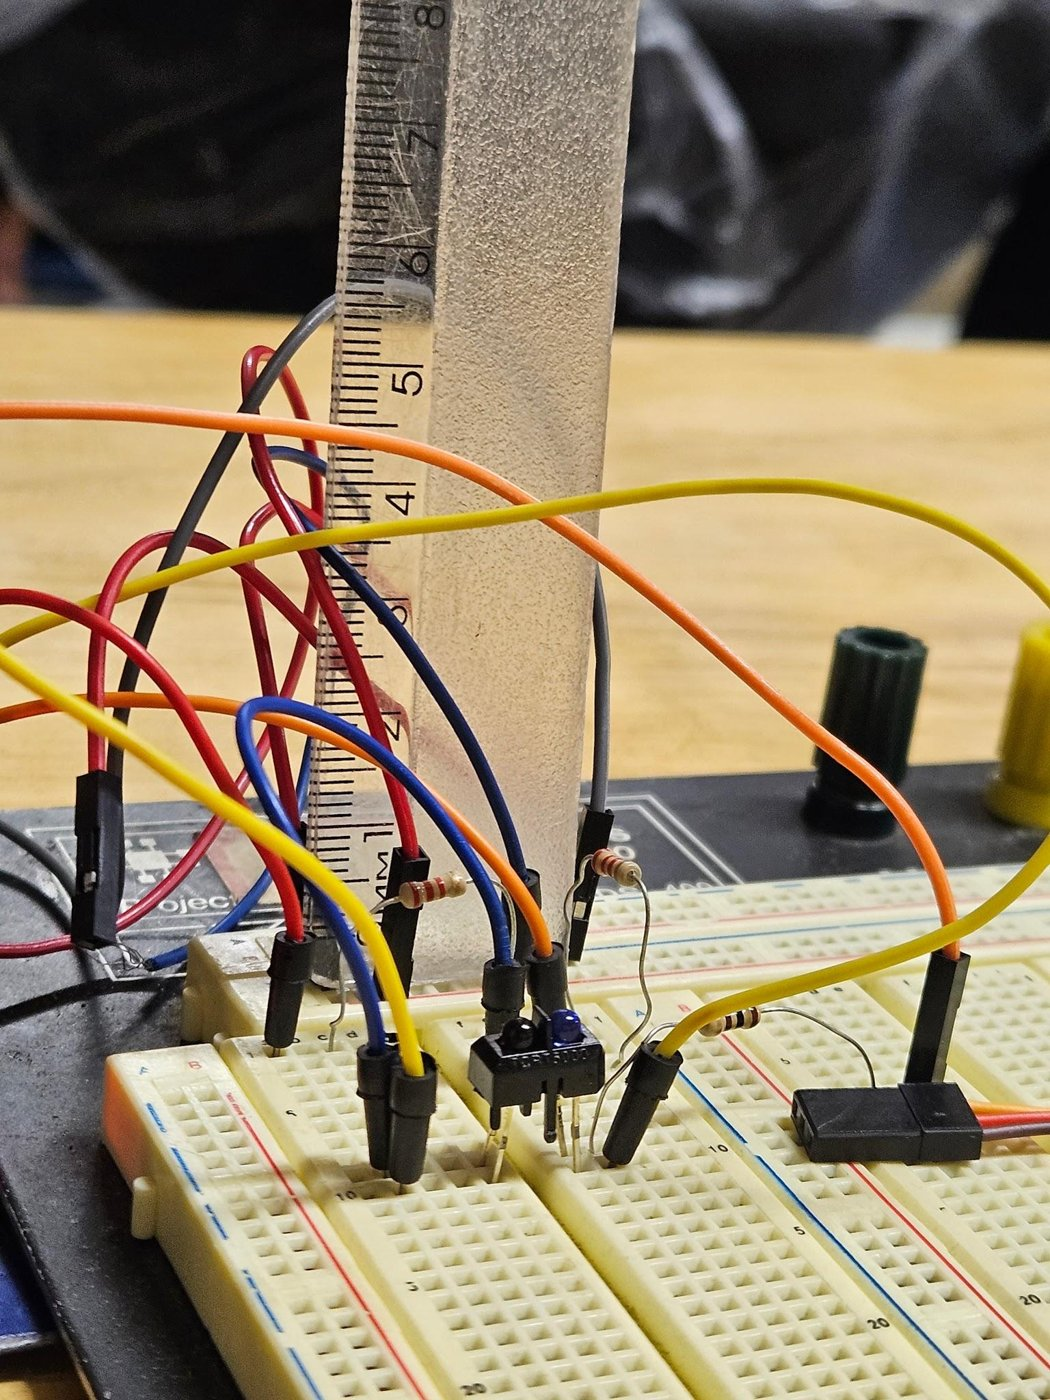
\includegraphics[width=\linewidth,height=7.5cm,keepaspectratio]{montagem_detalhe.jpg}
    \caption{Detalhe da montagem: TCRT5000 na protoboard, voltado para cima, com a régua fixada na vertical.}
    \label{fig:montagem-detalhe}
  \end{minipage}\hfill
  \begin{minipage}[b]{0.48\textwidth}
    \centering
    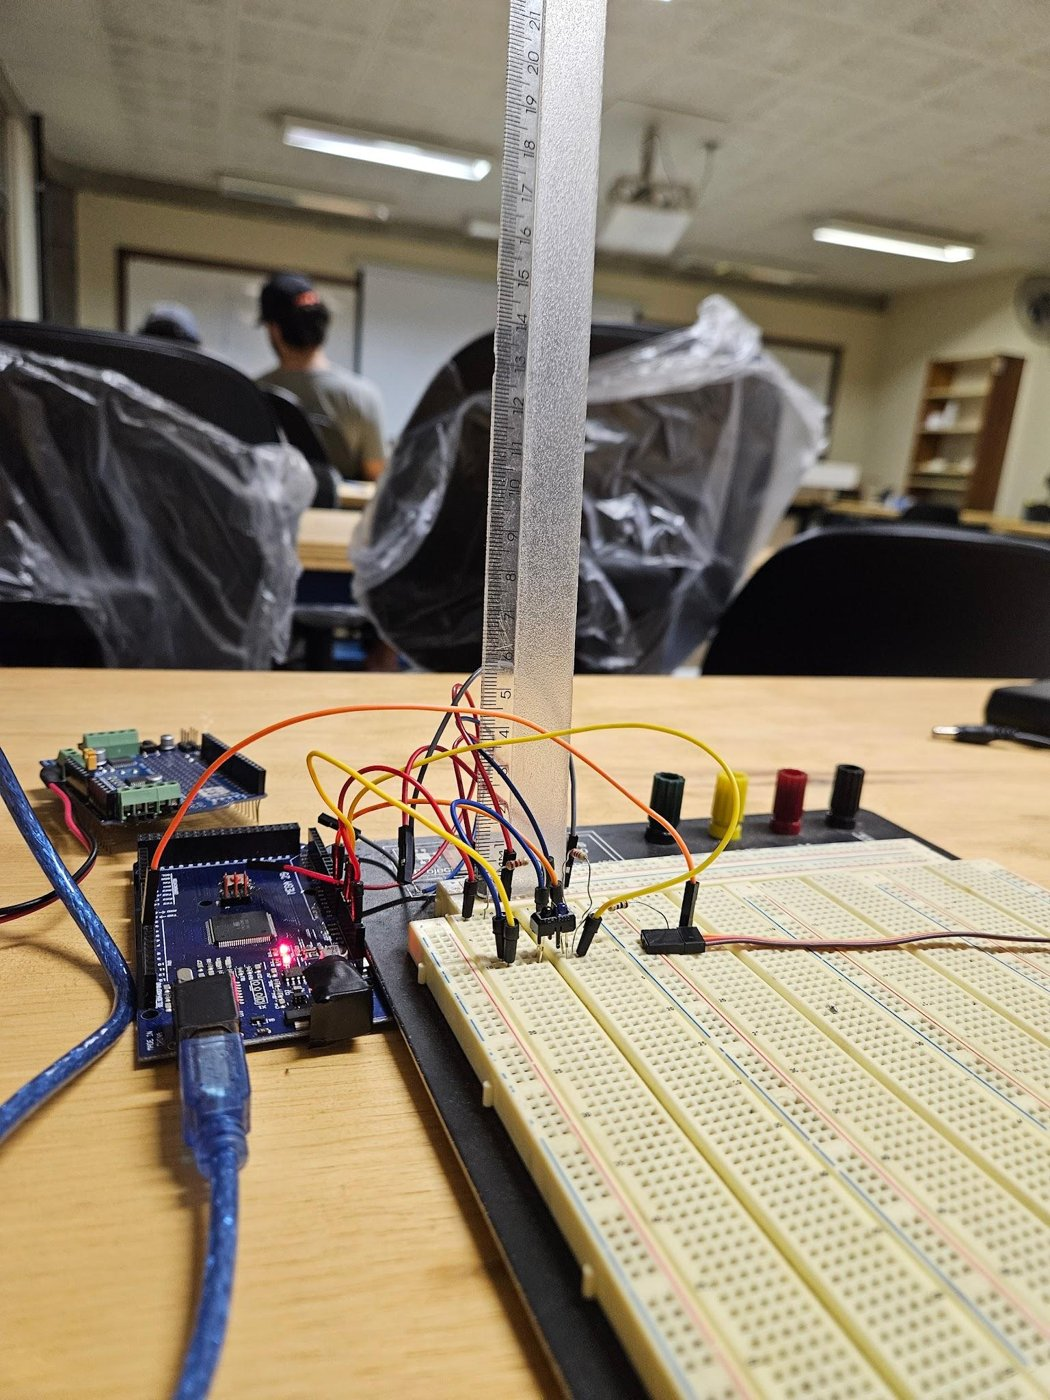
\includegraphics[width=\linewidth,height=7.5cm,keepaspectratio]{montagem_geral.jpg}
    \caption{Visão geral: Arduino Mega, protoboard e régua de 20~cm.}
    \label{fig:montagem-geral}
  \end{minipage}
\end{figure}

\begin{figure}[!htb]
  \centering
  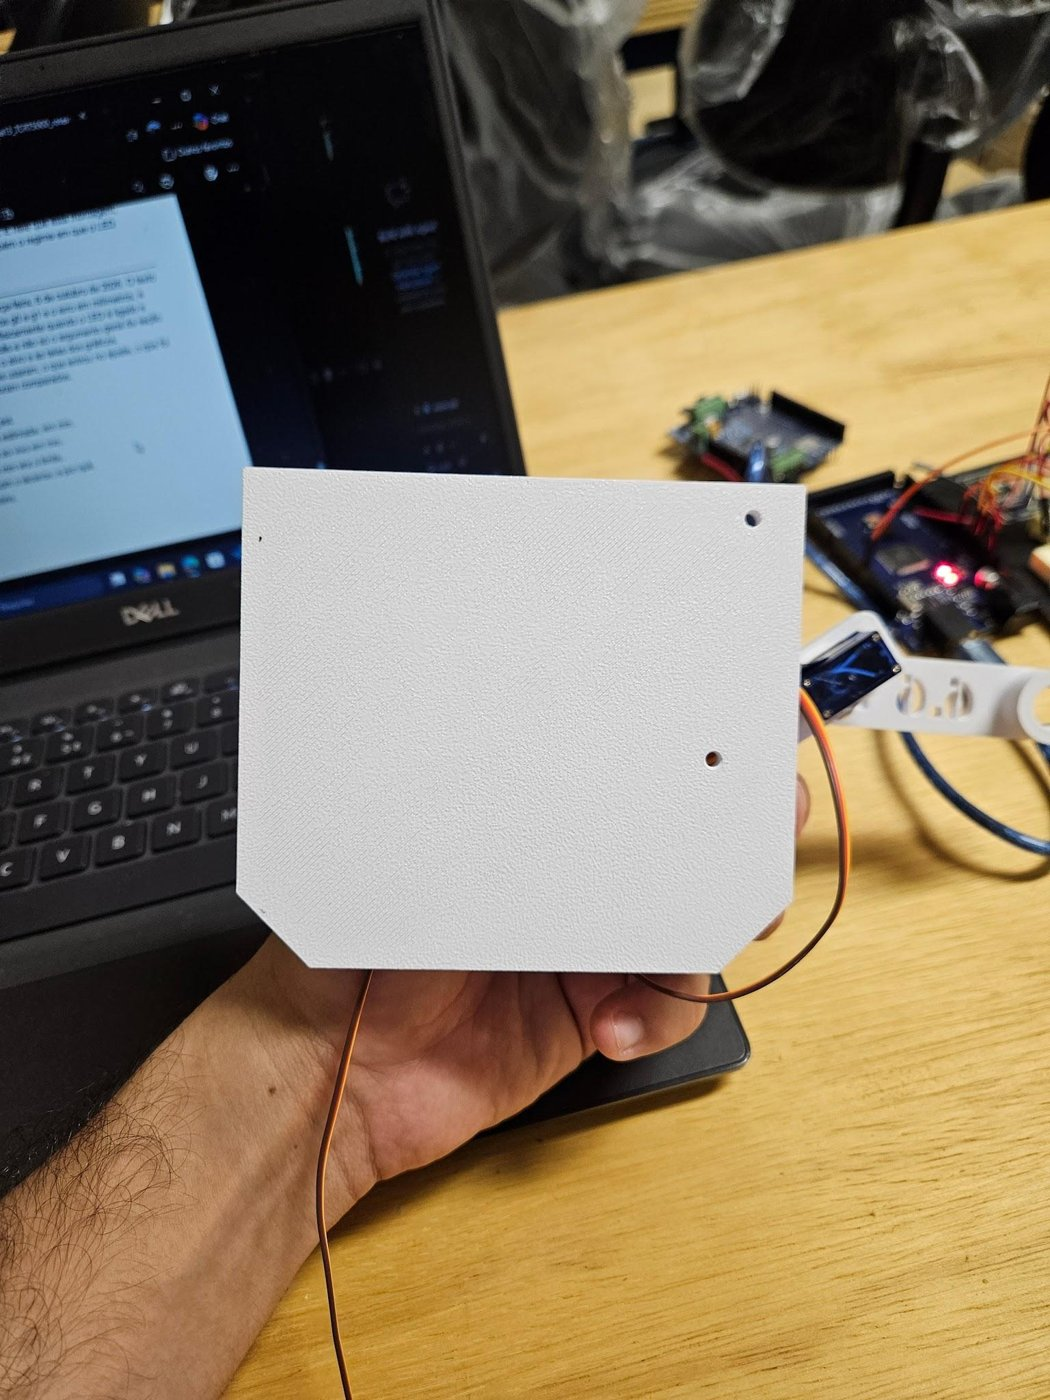
\includegraphics[height=7cm,keepaspectratio]{alvo.jpg}
  \caption{Alvo: placa branca de PLA impressa (base do braço mecânico).}
  \label{fig:alvo}
\end{figure}

% ------------------------------------------------------------------ 3
\section{Procedimento}

Medimos o sinal em 11 distâncias, de 0 a 200~mm em passos de 20~mm, com o LED aceso e apagado por 1000~ms. Fizemos duas séries de leitura (S e P), cada uma com uma leitura por distância.

\begin{enumerate}
  \item \textbf{Firmware.} Gravamos o sketch do roteiro com $t_{\mathrm{on}} = t_{\mathrm{off}} = 1000$~ms. A cada ciclo de 2~s, ele mede o A0 com o LED aceso ($\mathrm{adc}_{\mathrm{on}}$) e apagado ($\mathrm{adc}_{\mathrm{off}}$) e imprime $S$ na serial a 115\,200~baud.
  \item \textbf{Verificação.} Ao aproximar o alvo, vimos $S$ subir, o que confirmou a polaridade dos terminais e os resistores.
  \item \textbf{Caracterização.} Posicionamos o alvo a 0, 20, 40, \ldots, 200~mm da face do sensor, pela régua, e anotamos o sinal da serial. Registramos as duas séries na planilha como S (aba ``Arduino'') e P (aba ``Python'').
  \item \textbf{Fundo.} Sem alvo, lemos $S = 0$ ou $1$ na serial (Figura~\ref{fig:serial}). Esse é o nível de fundo usado para definir o alcance.
  \item \textbf{Ajuste.} Na planilha, calculamos $z = 1/\sqrt{S}$ e ajustamos $d$ contra $z$ por mínimos quadrados (funções \cod{SLOPE} e \cod{INTERCEPT}). O primeiro ajuste, com os 11 pontos da série S, deu os ganhos gravados no firmware.
  \item \textbf{Modelo no Arduino.} Gravamos $g_0$ e $g_1$ no sketch, que passou a imprimir \cod{sinal,mm}. Em seguida, aproximamos e afastamos o alvo com o \cod{plot\_serial.py} aberto.
  \item \textbf{Tempos de acionamento.} Repetimos a observação com $t_{\mathrm{on}} = t_{\mathrm{off}} = 1000$, 100, 10 e 1~ms.
\end{enumerate}

\paragraph{Faixa do ajuste.} O modelo vale onde o sinal ainda cai com a distância, longe da saturação e acima do fundo. Por isso, além do ajuste com os 11 pontos, fizemos um segundo ajuste restrito a 20 a 180~mm. Ele deixa de fora o ponto de 0~mm, que é contato com a face do sensor e onde as duas séries discordam em mais de 3 vezes (292 e 982), e o de 200~mm, com $S = 2$, a 1 ou 2 contagens do fundo. A Seção~\ref{sec:modelo} compara os dois.

% ------------------------------------------------------------------ 4
\section{Modelo e calibração}
\label{sec:modelo}

O modelo inverso reproduz a distância com RMSE de 8,6~mm (ganhos do firmware) a 7,0~mm (reajuste) na faixa de 20 a 180~mm.

\subsection{Modelo}

A luz refletida por um alvo difuso cai, em primeira aproximação, com o quadrado da distância. Invertendo essa relação, a distância fica linear em $z = 1/\sqrt{S}$:
\begin{equation}
  S(d) = \frac{\alpha}{d^2}
  \quad\Longrightarrow\quad
  d = g_0 + g_1\, z, \qquad z = \frac{1}{\sqrt{S}}.
  \label{eq:modelo}
\end{equation}
O ganho $g_1$ (mm$\cdot$cont$^{1/2}$) faz o papel de $\sqrt{\alpha}$. O intercepto $g_0$ (mm) absorve o zero da régua, o tamanho finito do alvo e o resíduo de luz ambiente.

\subsection{Dados e ajuste}

A Tabela~\ref{tab:dados} traz as duas séries, o $z$ da série S e a distância estimada com dois pares de ganhos. O primeiro par é o gravado no firmware (ajuste de 0 a 200~mm). O segundo é o reajuste em 20 a 180~mm, ambos sobre a série S. O erro é $d_{\mathrm{est}} - d$.

\begin{table}[!htb]
\centering
\small
\caption{Leituras, transformação $z$ e distância estimada com os dois pares de ganhos (série S).}
\label{tab:dados}
\begin{tabular}{rrrrrrrr}
\toprule
 & & & & \multicolumn{2}{c}{Firmware (0--200 mm)} & \multicolumn{2}{c}{Reajuste (20--180 mm)} \\
\cmidrule(lr){5-6}\cmidrule(lr){7-8}
$d$ (mm) & S & P & $z$ (S) & $d_{\mathrm{est}}$ (mm) & erro (mm) & $d_{\mathrm{est}}$ (mm) & erro (mm) \\
\midrule
200 & 2   & 2   & 0,7071 & 219,7 & $+19{,}7$ & 229,3 & $+29{,}3$ \\
180 & 3   & 3   & 0,5774 & 180,0 & $0{,}0$   & 188,0 & $+8{,}0$ \\
160 & 4   & 4   & 0,5000 & 156,3 & $-3{,}7$  & 163,3 & $+3{,}3$ \\
140 & 6   & 7   & 0,4082 & 128,2 & $-11{,}8$ & 134,1 & $-5{,}9$ \\
120 & 8   & 9   & 0,3536 & 111,5 & $-8{,}5$  & 116,7 & $-3{,}3$ \\
100 & 14  & 13  & 0,2673 & 85,1  & $-14{,}9$ & 89,2  & $-10{,}8$ \\
80  & 19  & 20  & 0,2294 & 73,5  & $-6{,}5$  & 77,1  & $-2{,}9$ \\
60  & 36  & 36  & 0,1667 & 54,3  & $-5{,}7$  & 57,1  & $-2{,}9$ \\
40  & 75  & 66  & 0,1155 & 38,6  & $-1{,}4$  & 40,8  & $+0{,}8$ \\
20  & 115 & 190 & 0,0933 & 31,8  & $+11{,}8$ & 33,7  & $+13{,}7$ \\
0   & 292 & 982 & 0,0585 & 21,1  & $+21{,}1$ & 22,7  & $+22{,}7$ \\
\bottomrule
\end{tabular}
\end{table}

\begin{table}[!htb]
\centering
\small
\caption{Ganhos e erro dos dois ajustes. O RMSE é calculado na faixa de 20 a 180~mm.}
\label{tab:ganhos}
\setlength{\tabcolsep}{4pt}
\begin{tabular}{lrrrrrr}
\toprule
Ajuste (série S) & Pontos & $g_0$ (mm) & $g_1$ (mm$\cdot$cont$^{1/2}$) & $R^2$ & RMSE S (mm) & RMSE P (mm) \\
\midrule
Firmware (0--200 mm)  & 11 & 3,22 & 306,18 & 0,966 & 8,6 & 10,3 \\
Reajuste (20--180 mm) & 9  & 4,03 & 318,56 & 0,982 & 7,0 & 7,9 \\
\bottomrule
\end{tabular}
\end{table}

A série P não entrou em nenhum dos dois ajustes e serve de validação. O reajuste também erra menos nela (7,9 contra 10,3~mm), o que mostra que o ganho não vem só de ajustar melhor os mesmos pontos.

Os dois pontos extremos pesam bastante no ajuste com os 11 pontos. Com eles, a reta estima de 6 a 15~mm a menos na faixa de 60 a 140~mm (viés médio de $-4{,}5$~mm). O ajuste em 20 a 180~mm tem viés nulo na faixa usada. Nele, os maiores desvios ficam a 20~mm ($+13{,}7$~mm) e a 100~mm ($-10{,}8$~mm).

\paragraph{Expoente real.} Uma reta em escala log-log entre 20 e 180~mm dá $S \propto d^{-1{,}74}$ na série S e $S \propto d^{-1{,}86}$ na série P. A queda é mais suave que o inverso do quadrado (expoente $-2$). O desvio se concentra perto do sensor: a 20~mm, o sinal medido fica abaixo do previsto. Nessa distância, o cone de emissão do LED e o campo de visão do fototransistor ainda não se sobrepõem por inteiro.

\begin{figure}[!htb]
  \centering
  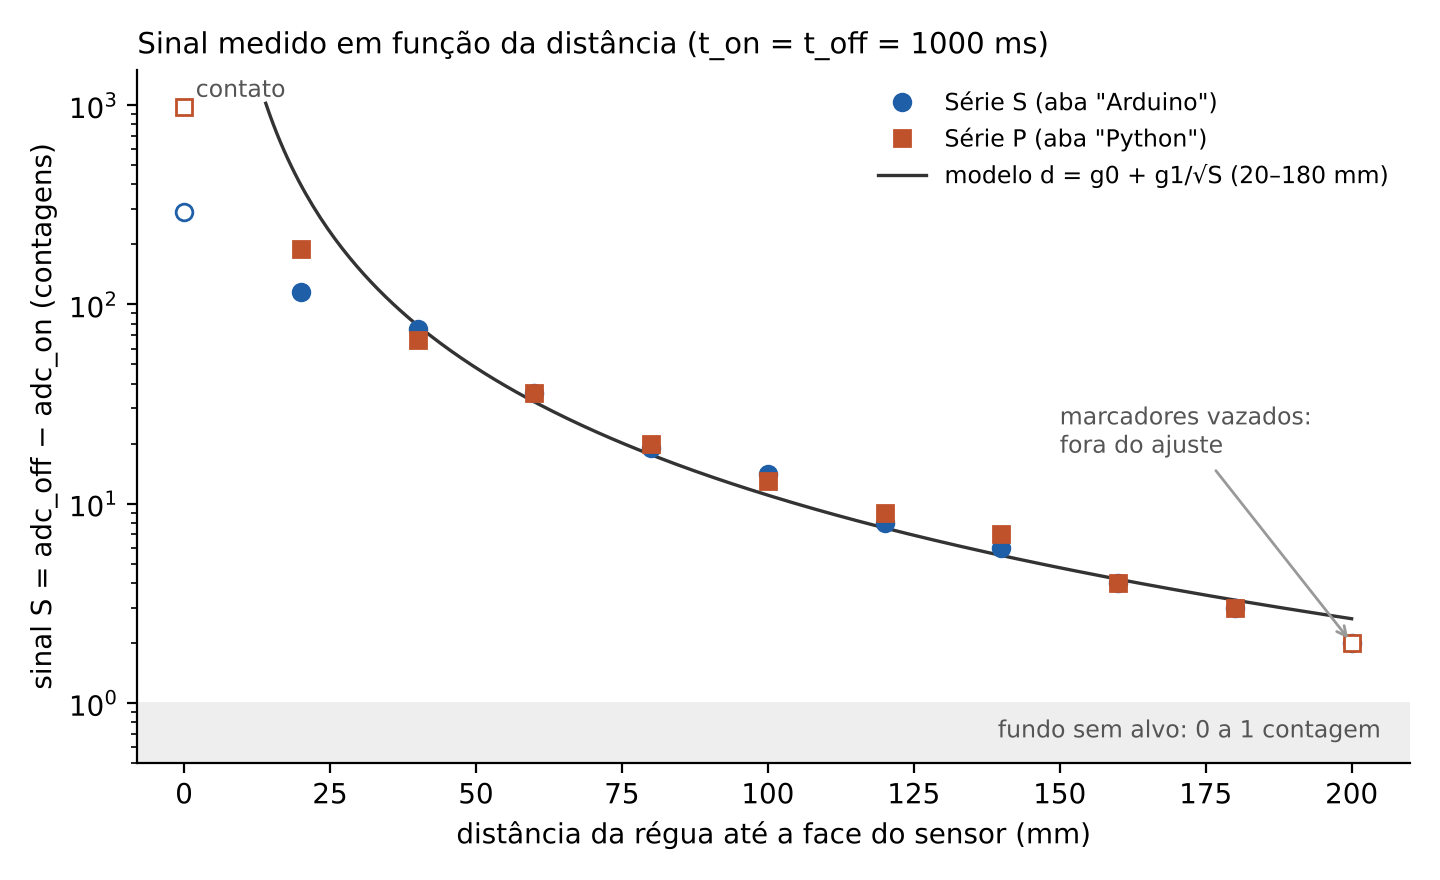
\includegraphics[width=0.85\textwidth]{fig_sinal_distancia.png}
  \caption{Sinal $S$ em função da distância da régua (escala logarítmica). Marcadores cheios: pontos do reajuste; vazados: excluídos. A curva é o modelo reajustado; a faixa cinza é o fundo sem alvo.}
  \label{fig:sinal}
\end{figure}

\begin{figure}[!htb]
  \centering
  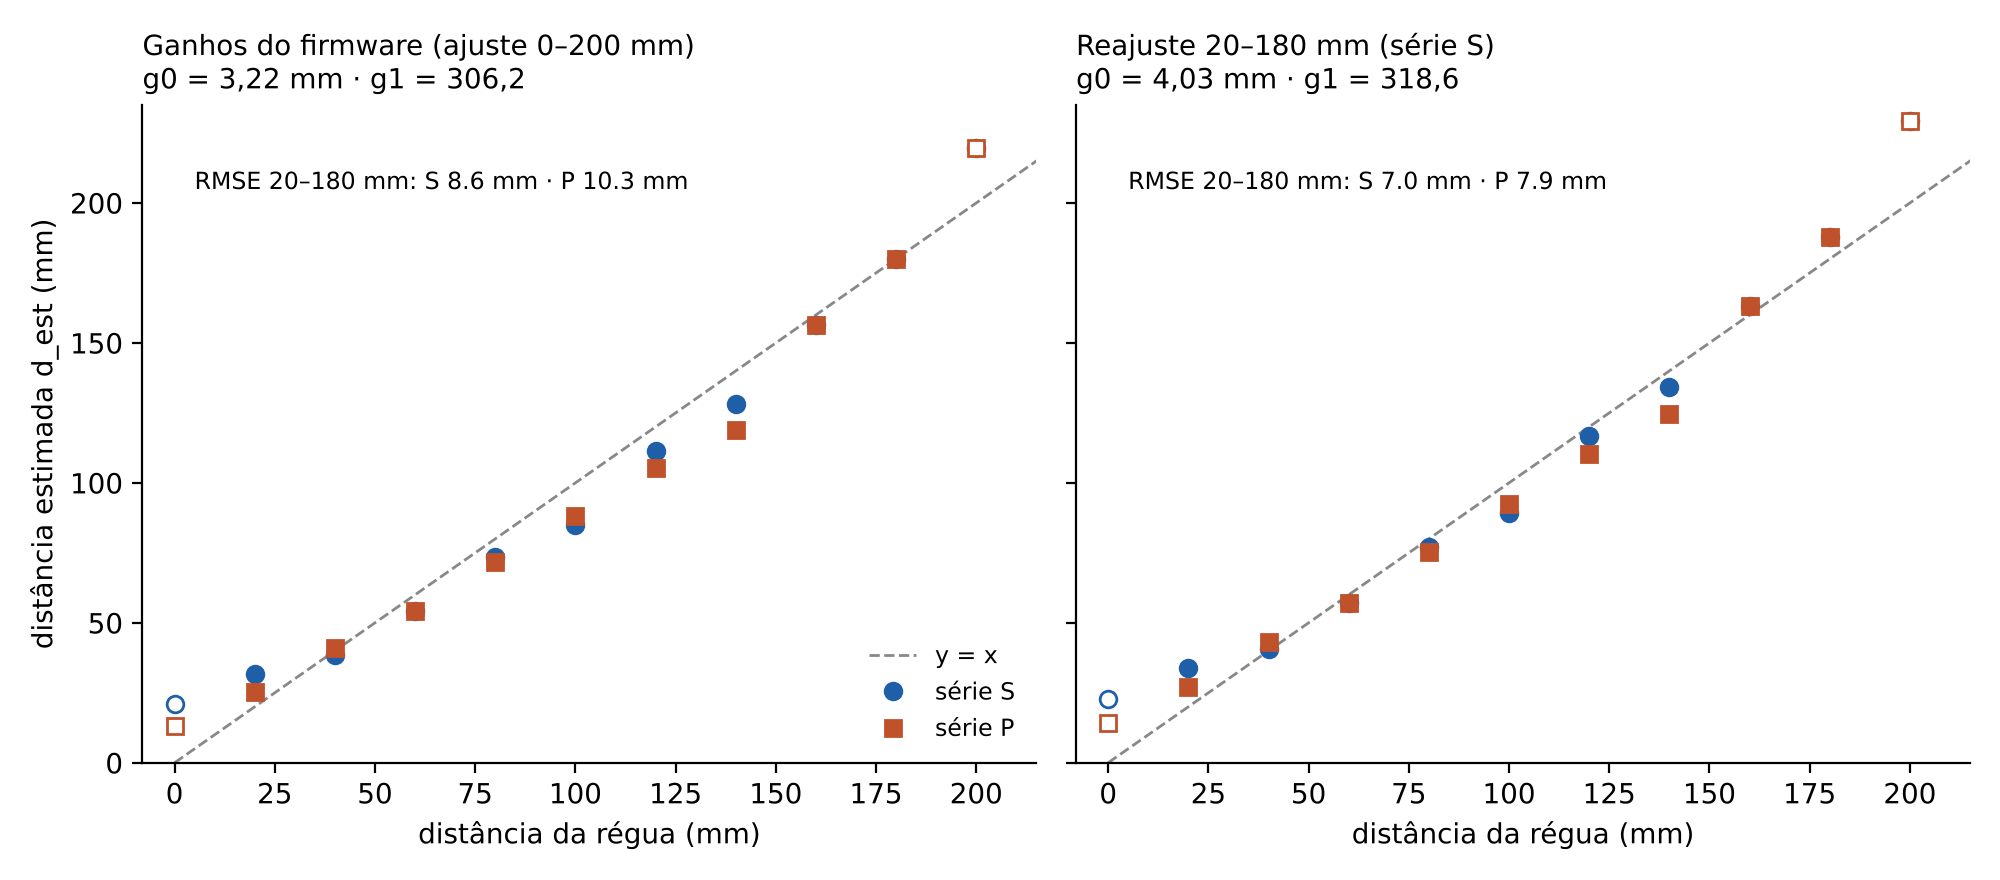
\includegraphics[width=\textwidth]{fig_dest_vs_d.png}
  \caption{Distância estimada contra a distância da régua, com a reta $y = x$. À esquerda, os ganhos do firmware; à direita, o reajuste em 20 a 180~mm.}
  \label{fig:dest}
\end{figure}

% ------------------------------------------------------------------ 5
\section{Resultados}

O sinal ficou acima do fundo em toda a faixa de 0 a 200~mm, mas a 200~mm a diferença foi de só 1 a 2 contagens. A partir de 160~mm, uma contagem a mais ou a menos muda a estimativa em 16~mm ou mais.

\subsection{Alcance}
\label{sec:alcance}

Com 1000~ms de acionamento e a placa branca, o sinal caiu de forma monótona em toda a faixa medida: de 115 a 190 contagens a 20~mm até 2 contagens a 200~mm (Figura~\ref{fig:sinal}). Sem alvo, lemos $S = 0$ ou $1$. A 200~mm, portanto, o sinal ainda se separa do fundo, mas por apenas 1 a 2 contagens.

Observamos leituras estáveis até cerca de 160~mm ($S = 4$). Entre 160 e 200~mm, a estimativa oscilou e, em algumas leituras, $S$ caiu a 0 ou 1. Assim, 200~mm é o limite de detecção desta montagem, e o alcance útil, em que a leitura se repete, fica em torno de 160~mm.

O alcance depende da refletância do alvo: a superfície branca e fosca da placa devolve ao detector uma fração maior da luz do que um alvo escuro ou espelhado, que espalharia a luz para fora do campo de visão.

\subsection{Repetibilidade entre as séries}

Nas duas séries, os sinais coincidem ou diferem em 1 contagem de 60 a 200~mm. As diferenças grandes aparecem perto do sensor: 75 contra 66 a 40~mm (13\%), 115 contra 190 a 20~mm (49\%) e 292 contra 982 no contato. Perto do contato, pequenas mudanças de ângulo e de posição do alvo mudam muito a luz que volta ao detector.

\subsection{Sinal em tensão e em corrente}

Cada contagem do conversor de 10 bits com referência de 5~V vale $5/1023 \approx 4{,}89$~mV. Dividindo pela resistência de \emph{pull-up}, obtemos a variação da corrente de coletor causada pela luz refletida (Tabela~\ref{tab:sensibilidade}).

\begin{table}[!htb]
\centering
\small
\caption{Sinal da série S convertido em tensão ($\Delta V = S \cdot 4{,}89$~mV) e em corrente de coletor ($\Delta I = \Delta V / 4{,}0~\mathrm{k}\Omega$).}
\label{tab:sensibilidade}
\begin{tabular}{rrrr}
\toprule
$d$ (mm) & $S$ (contagens) & $\Delta V$ (mV) & $\Delta I$ ($\mu$A) \\
\midrule
200 & 2   & 9,8   & 2,4 \\
160 & 4   & 19,6  & 4,9 \\
100 & 14  & 68,4  & 17,1 \\
60  & 36  & 176,0 & 44,0 \\
40  & 75  & 366,6 & 91,7 \\
20  & 115 & 562,2 & 140,5 \\
\bottomrule
\end{tabular}
\end{table}

A 200~mm, a luz que volta ao detector muda a corrente de coletor em apenas 2,4~$\mu$A, contra 38~mA no emissor: uma razão da ordem de $10^{-4}$. A 20~mm, a variação chega a 141~$\mu$A, ainda longe de saturar o fototransistor, cuja corrente máxima com 4,0~k$\Omega$ seria de cerca de 1,25~mA. A saturação só aparece no contato, onde a série P chegou a 982 contagens, perto do fundo de escala.

\subsection{Resolução}
\label{sec:resolucao}

O conversor entrega inteiros, então a distância estimada só assume valores discretos. Com os ganhos do firmware, uma contagem a mais ou a menos muda a estimativa conforme a Tabela~\ref{tab:resolucao}.

\begin{table}[!htb]
\centering
\small
\caption{Salto da distância estimada quando $S$ varia uma contagem (ganhos do firmware).}
\label{tab:resolucao}
\begin{tabular}{ccc}
\toprule
Faixa de $S$ & Distância estimada (mm) & Salto por contagem (mm) \\
\midrule
1 $\to$ 2   & 309 $\to$ 220 & 90 \\
2 $\to$ 3   & 220 $\to$ 180 & 40 \\
3 $\to$ 4   & 180 $\to$ 156 & 24 \\
4 $\to$ 5   & 156 $\to$ 140 & 16 \\
8 $\to$ 9   & 111 $\to$ 105 & 6 \\
19 $\to$ 20 & 73 $\to$ 72   & 2 \\
36 $\to$ 37 & 54 $\to$ 54   & 0,7 \\
\bottomrule
\end{tabular}
\end{table}

Acima de cerca de 120~mm, o erro de quantização passa a ser maior que o erro do modelo (7 a 9~mm). Por isso, uma oscilação de $\pm1$ contagem, normal em qualquer leitura analógica, aparece como saltos de dezenas de milímetros no fim da faixa (Figuras~\ref{fig:resolucao} e~\ref{fig:curva}).

\begin{figure}[!htb]
  \centering
  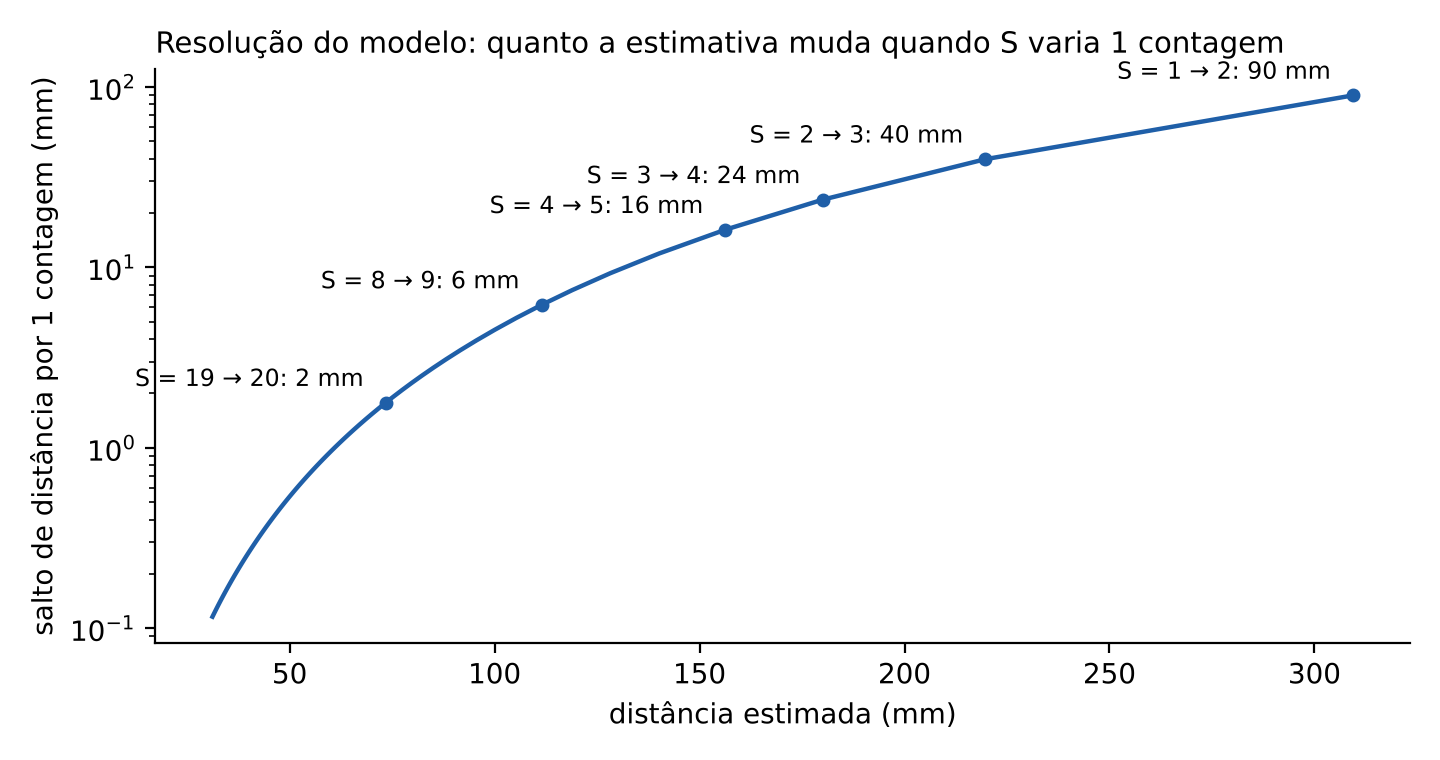
\includegraphics[width=0.85\textwidth]{fig_resolucao.png}
  \caption{Salto da distância estimada quando $S$ varia uma contagem, com os ganhos do firmware.}
  \label{fig:resolucao}
\end{figure}

% ------------------------------------------------------------------ 6
\section{Firmware e curva ao vivo}

O sketch imprime \cod{sinal,mm} em cada ciclo, calculando $d = g_0 + g_1/\sqrt{S}$ com $g_0 = 3{,}22$~mm e $g_1 = 306{,}18$. A saída serial confirma os ganhos gravados: $S = 1$ dá 309,4~mm, $S = 2$ dá 219,7~mm e $S = 387$ dá 18,8~mm, exatamente como na Equação~\eqref{eq:modelo} (Figura~\ref{fig:serial}).

O roteiro pede que $S = 0$ não gere divisão por zero e que o sketch imprima um valor justificável. Pela Seção~\ref{sec:alcance}, $S = 0$ só ocorre além de cerca de 200~mm, onde o modelo já não vale. Por isso, o sketch que acompanha este relatório (Apêndice~\ref{ap:sketch}) imprime $-1$ nesse caso: um valor impossível como distância, que marca a leitura como fora de alcance e que o \cod{plot\_serial.py} descarta. Na captura da Figura~\ref{fig:serial}, essas leituras aparecem como \cod{0,inf}.

Para a curva ao vivo, adaptamos o \cod{plot\_serial.py} do roteiro para ler a segunda coluna de cada linha (a distância) e desenhá-la em milímetros. Com o script aberto, aproximamos o alvo do sensor, afastamos além de 200~mm e aproximamos de novo (Figura~\ref{fig:curva}).

A curva sobe e desce de forma suave abaixo de cerca de 130~mm. Acima disso, alterna em degraus entre 140, 156, 180, 220 e 309~mm, que são justamente as distâncias de $S = 5$, 4, 3, 2 e 1 na Tabela~\ref{tab:resolucao}. Os picos e as oscilações no topo da curva são, portanto, o sinal oscilando $\pm1$ contagem na região em que cada contagem vale dezenas de milímetros. Não são falhas do modelo.

\begin{figure}[!htb]
  \centering
  \begin{minipage}[t]{0.40\textwidth}
    \centering
    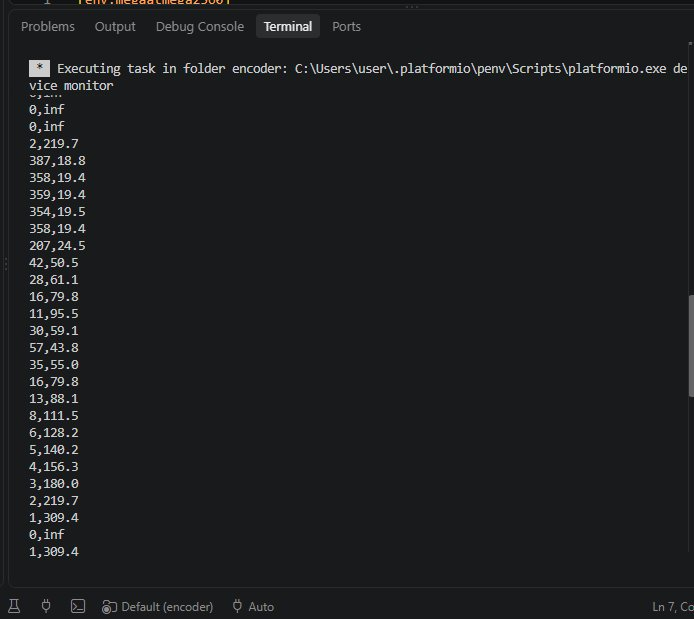
\includegraphics[width=\linewidth,height=9cm,keepaspectratio]{serial.jpg}
    \caption{Saída serial no formato \cod{sinal,mm}. As linhas com sinal 0 são leituras sem alvo.}
    \label{fig:serial}
  \end{minipage}\hfill
  \begin{minipage}[t]{0.56\textwidth}
    \centering
    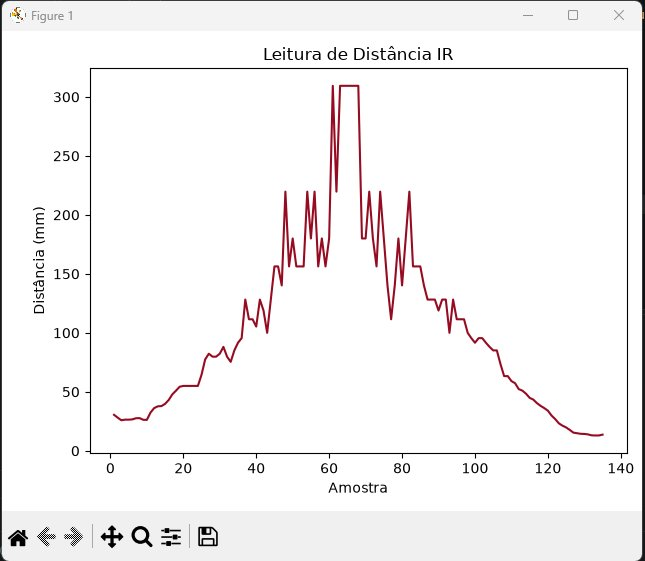
\includegraphics[width=\linewidth,height=9cm,keepaspectratio]{curva_ao_vivo.jpg}
    \caption{Curva ao vivo da distância estimada (\cod{plot\_serial.py}), com o alvo sendo afastado além de 200~mm e aproximado de novo.}
    \label{fig:curva}
  \end{minipage}
\end{figure}

% ------------------------------------------------------------------ 7
\section{Discussão}

\subsection{Até onde o sensor enxerga}

Nesta montagem, 200~mm é o limite, e não um ponto de folga. A 200~mm restam 2 contagens contra um fundo de 0 a 1. A distância seguinte que o modelo conseguiria representar, $S = 1$, corresponde a 309~mm e já se confunde com o fundo.

O alcance útil é menor que o alcance de detecção. A partir de 160~mm, uma contagem vale de 16 a 40~mm, e uma oscilação normal de $\pm1$ contagem tira a estimativa da faixa da régua. O roteiro lembra que a folha de dados concentra a resposta útil em poucos centímetros, com pico perto de 2,5~mm. O alcance maior que obtivemos vem do regime de 1~s, do alvo branco grande e da corrente de 38~mA no emissor. Mesmo assim, o sinal a 200~mm é menos de 0,2\% da escala do conversor.

\subsection{O que a redução dos tempos fez com o sinal}

Ao reduzir $t_{\mathrm{on}}$ e $t_{\mathrm{off}}$ de 1000~ms para 100, 10 e 1~ms, observamos que as leituras ficaram menos estáveis e mais difíceis de separar do ruído, principalmente nas maiores distâncias. A análise abaixo usa nossas medidas de 1000~ms para mostrar por que o efeito aparece primeiro no fim da faixa.

Fisicamente, quando o D8 sobe, o LED não atinge a potência óptica final no mesmo instante. Os portadores levam de dezenas a centenas de microssegundos para se estabelecer na junção. No fototransistor, os fótons geram portadores na base, e a corrente de coletor cresce com o ganho do transistor. Quando o LED apaga, a carga armazenada ainda sustenta corrente por algum tempo. A capacitância da junção, carregada pelo resistor de \emph{pull-up}, define uma constante de tempo: quanto maior o resistor, mais lenta a resposta.

Se a janela é curta, $\mathrm{adc}_{\mathrm{on}}$ é lido antes de o par emissor--detector chegar ao regime, e $\mathrm{adc}_{\mathrm{off}}$ é lido enquanto o coletor ainda conduz. A diferença $S$ encolhe, mas o ruído da leitura continua da ordem de 1 contagem.

Nossas medidas mostram por que isso derruba o alcance justamente no fim da faixa. Uma redução de 25\% em $S$ tira 1 contagem a 160~mm (de 4 para 3), o que desloca a estimativa em 24~mm. A 60~mm, a mesma redução tira 9 contagens (de 36 para 27), o que desloca a estimativa em cerca de 8~mm. A 200~mm, ela leva $S$ de 2 a 1 ou a 0, que já é o fundo. Com tempos curtos, portanto, o alcance encolhe primeiro na ponta, como observamos.

Uma segunda causa que pode contribuir é a cintilação da iluminação fluorescente da sala, a 120~Hz (período de 8,3~ms). Com $t_{\mathrm{on}}$ e $t_{\mathrm{off}}$ de 1 a 10~ms, $\mathrm{adc}_{\mathrm{on}}$ e $\mathrm{adc}_{\mathrm{off}}$ caem em fases diferentes desse ciclo. A subtração deixa de cancelar a luz ambiente e soma à diferença a componente infravermelha que passa pelo filtro. Com 1000~ms, o efeito existe, mas é uma oscilação aleatória de fundo, sem tendência.

\subsection{Fontes de desvio do modelo}

\begin{itemize}
  \item \textbf{Quantização.} Acima de 120~mm, é a maior fonte de erro (Seção~\ref{sec:resolucao}). O erro de arredondamento de meia contagem tem variância $q^2/12$, como na análise de quantização da aula de filtros. Em distância, como $\lvert \mathrm{d}d/\mathrm{d}S \rvert = d^3/(2g_1^2)$, o mesmo erro de contagem cresce com o cubo da distância.
  \item \textbf{Faixa do ajuste.} Os pontos de contato (0~mm) e de 200~mm deslocam a reta e geram um viés de $-4{,}5$~mm na faixa útil. Restringir o ajuste a 20 a 180~mm elimina esse viés e reduz o RMSE de 8,6 para 7,0~mm.
  \item \textbf{Forma do modelo.} O sinal cai como $d^{-1{,}7}$ a $d^{-1{,}9}$, não como $d^{-2}$. O desvio é maior perto do sensor, onde a geometria do emissor e do detector pesa mais. Por isso o erro a 20~mm é de $+12$ a $+14$~mm nos dois ajustes.
  \item \textbf{Ângulo e posição do alvo.} Perto do sensor, uma pequena inclinação muda bastante a luz que volta ao detector. É ali que as duas séries mais diferem (49\% a 20~mm).
\end{itemize}

\subsection{Limitações do sensor e do método}

\begin{itemize}
  \item \textbf{Alcance útil.} A resolução piora com o cubo da distância. Por isso, a montagem detecta o alvo até 200~mm, mas só mede com repetibilidade até cerca de 160~mm.
  \item \textbf{Faixa dinâmica.} A 200~mm, o sinal ocupa menos de 0,2\% da escala do conversor, então uma variação de 1 contagem pesa muito.
  \item \textbf{Modelo.} O inverso do quadrado é uma aproximação. Perto do sensor, a geometria do emissor e do detector afasta a curva real do modelo, e o desvio chega a $+14$~mm a 20~mm.
  \item \textbf{Dependência do alvo e do ambiente.} Os ganhos valem para a placa branca, 38~mA no LED, 1000~ms de acionamento e a iluminação da sala. Outro alvo ou outra luz ambiente exigem nova calibração.
\end{itemize}

% ------------------------------------------------------------------ 8
\section{Conclusão}

O TCRT5000 funcionou como sensor de distância de 20 a 180~mm, com o modelo $d = g_0 + g_1/\sqrt{S}$ embarcado no Arduino e erro RMS de 8,6~mm com os ganhos gravados ($g_0 = 3{,}22$~mm, $g_1 = 306{,}2$). Com 1000~ms de acionamento e alvo branco, o sinal se separou do fundo até 200~mm, o limite desta montagem, e as leituras foram confiáveis até cerca de 160~mm. Reduzir os tempos de acionamento piorou primeiro as leituras distantes, onde cada contagem perdida vale dezenas de milímetros.

Como próximos passos, propomos:
\begin{enumerate}
  \item gravar no firmware os ganhos do ajuste em 20 a 180~mm ($g_0 = 4{,}03$~mm, $g_1 = 318{,}56$), que reduzem o RMSE para 7,0~mm;
  \item fazer a média de várias conversões por ciclo, o que reduz o efeito da quantização no fim da faixa;
  \item aumentar o \emph{pull-up} para elevar o sinal nas maiores distâncias, verificando que o fototransistor não sature perto do sensor;
  \item montar o alvo num suporte com ajuste de ângulo, para estender a caracterização a alvos de outras cores e inclinações.
\end{enumerate}

% ------------------------------------------------------------------ 9
\section{Arquivos}

A planilha e o sketch final acompanham este relatório, como pede o roteiro.

\begin{table}[!htb]
\centering
\small
\begin{tabularx}{\textwidth}{>{\raggedright\arraybackslash}p{6.2cm}X}
\toprule
Arquivo & Conteúdo \\
\midrule
\cod{calibracao\_tcrt5000.xlsx} & leituras das séries S e P, $z = 1/\sqrt{S}$, $g_0$, $g_1$, $R^2$, $d_{\mathrm{est}}$ e erro para os dois ajustes, e tabela de resolução \\
\cod{tcrt5000\_distancia/src/main.cpp} & sketch que imprime \cod{sinal,mm} com os ganhos da calibração e trata $S = 0$ (Apêndice~\ref{ap:sketch}) \\
\cod{plot\_serial.py} & gráfico ao vivo da segunda coluna da serial (distância em mm) \\
\bottomrule
\end{tabularx}
\end{table}

% ------------------------------------------------------------------ referências
\begin{thebibliography}{9}
\bibitem{roteiro} REZECK, P. \emph{Sensor de distância por infravermelho --- TCRT5000 na protoboard} (roteiro da Aula 13). Projeto de Sistemas Robóticos, DCC/UFMG, 2026.
\bibitem{filtros} REZECK, P. \emph{Filtros} (slides): quantização e variância $q^2/12$. Projeto de Sistemas Robóticos, DCC/UFMG, 2026.
\bibitem{vishay} VISHAY SEMICONDUCTORS. \emph{TCRT5000, TCRT5000L --- Reflective Optical Sensor with Transistor Output} (folha de dados), citada no roteiro para o pico de resposta perto de 2,5~mm.
\end{thebibliography}

% ------------------------------------------------------------------ apêndice
\appendix
\section{Sketch}
\label{ap:sketch}

\lstinputlisting{codigo/main.cpp}

\end{document}
